\documentclass[12pt,a4paper]{article}
\usepackage[utf8]{inputenc}
\usepackage[T1]{fontenc}
\usepackage[brazilian]{babel}
\usepackage{amsmath,amssymb}
\usepackage{graphicx}
\usepackage{booktabs}
\usepackage{geometry}
\geometry{margin=2.5cm}
\usepackage{hyperref}

\title{NDVI de satélite na predição de surtos de dengue no Brasil:\\
um resultado nulo rigoroso com dados públicos abertos}
\author{Sistema AI Cientista BR\thanks{Manuscrito gerado por pipeline multiagente
com roteamento MoE; números injetados dos artefatos do experimento.}}
\date{\today}

\begin{document}
\maketitle

\begin{abstract}
\textbf{Objetivo.} Testar se a adição de atributos de vegetação por satélite
(NDVI/MODIS) melhora a predição de surtos de dengue em municípios brasileiros,
sobre dados públicos abertos e sem nenhum dado sintético.
\textbf{Métodos.} Unimos o InfoDengue (Fiocruz/FGV), com 1233 semanas-município,
a NDVI real do NASA GIBS agregado por município (malha do IBGE) e por semana
epidemiológica. Comparamos três cenários sob validação estritamente temporal,
\texttt{seed}=42, IC~95\% por bootstrap (1000 reamostragens), teste de Wilcoxon
pareado e $d$ de Cohen.
\textbf{Resultados.} O cenário B (GB com satélite) obteve F1~=~0,9615
(IC~95\% [0,9254; 0,9877]), contra
F1~=~0,9434 do baseline A (regressão logística tabular) e
F1~=~0,9554 da ablação C (GB tabular). O efeito \emph{isolado} do satélite
(B vs C) foi $\Delta$F1~=~0,0049 e
$\Delta$F1~(B vs A)~=~0,0177, ambos abaixo do limiar
pré-registrado de 0,02. A análise de sensibilidade, sem os
atributos de nível de alerta, inverte o sinal: $\Delta$F1~(B vs C)~=~-0,0483.
\textbf{Conclusão.} Não rejeitar h0 (resultado nulo). O NDVI não melhorou a predição de
forma confiável, e o ganho aparente de B sobre A se deve à troca de algoritmo,
não ao satélite. Reportamos o resultado nulo como contribuição.
\end{abstract}

\section{Introdução}
A dengue é uma das arboviroses de maior carga no Brasil, e sistemas de alerta
precoce dependem de predição acurada de surtos. Trabalhos recentes usam
aprendizado de máquina com preditores climáticos e de sensoriamento remoto
\cite{10.1371/journal.pntd.0005973}\cite{10.1073/pnas.1909865116}\cite{10.1371/journal.pntd.0008056}. A hipótese comum é que a vegetação, capturada por
NDVI, sinaliza habitat do vetor e melhora a predição. Testamos essa hipótese de
forma pré-registrada, com dados públicos abertos e sem dados sintéticos.

\section{Trabalhos Relacionados}
Modelos de predição de dengue com aprendizado de máquina foram revisados
sistematicamente \cite{10.1038/srep33707}\cite{10.1016/j.physa.2019.121266}. Estudos comparam florestas aleatórias e redes
neurais \cite{10.1371/journal.pntd.0005729}, métodos híbridos \cite{10.1371/journal.pntd.0010509}, aprendizado profundo com clima
\cite{10.3390/ijerph17020453}\cite{10.1098/rsif.2016.0410} e superconjuntos de previsão \cite{10.1016/j.sste.2020.100372}. O uso de vegetação
derivada de satélite é central em \cite{10.1038/s41598-020-79193-2}\cite{10.1186/s12879-019-3874-x}. Nossa contribuição difere
ao (i) isolar o efeito do satélite com um cenário de ablação de mesmo algoritmo,
(ii) usar validação estritamente temporal e (iii) reportar o resultado nulo com
o mesmo rigor que um resultado positivo.

\textbf{Estado da arte (métricas extraídas dos abstracts originais).} A
Tabela~\ref{tab:sota} reúne as métricas reportadas por estudos comparáveis,
obtidas dos abstracts reais via Crossref/OpenAlex. O SOTA de referência mais
direto é o de Souza et al. (?), único estudo brasileiro
da lista, com \textbf{acurácia 0,80} sobre dados
exclusivamente climáticos. É contra esse patamar que nosso baseline tabular se
posiciona.

\begin{table}[h]
\centering
\caption{Estado da arte: métricas reportadas nos abstracts originais (Tarefa 1).}
\label{tab:sota}
\begin{tabular}{llrr}
\toprule
Estudo & Métrica & Valor (\%) & Ref. \\
\midrule
    Souza (2022) & acuracia & 0,80 & \cite{10.1016/j.eswa.2021.116324} \\
    Yavari Nejad (2021) & acuracia & 92,35 & \cite{10.1186/s12911-021-01493-y} \\
    Salim (2021) & acuracia & 70,00 & \cite{10.1038/s41598-020-79193-2} \\
    Iqbal (2019) & acuracia & 92,00 & \cite{10.31449/inf.v43i3.1548} \\
    Thirugnanam (2023) & F1 & 98,00 & \cite{10.18280/ria.370521} \\
\bottomrule
\end{tabular}
\end{table}

\section{Materiais}
\textbf{InfoDengue} (Fiocruz/FGV), \emph{versão da API} \texttt{alertcity},
semanas epidemiológicas observadas, \url{https://info.dengue.mat.br/api/alertcity}:
1233 amostras, 8 municípios, 8
atributos tabulares. Coleta: 2026-10-20T23:46:02.
\textbf{NASA GIBS/MODIS}, camada \texttt{MODIS\_Terra\_L3\_NDVI\_16Day}
(produto MOD13, composto de 16 dias), \url{https://gibs.earthdata.nasa.gov},
colormap oficial \texttt{MODIS\_L3\_NDVI.xml} (142 entradas RGB$\to$NDVI),
\url{https://gibs.earthdata.nasa.gov/colormaps/v1.0/MODIS\_L3\_NDVI.xml}:
4 atributos de satélite.
\textbf{Malha municipal} do IBGE, \url{https://servicodados.ibge.gov.br/api/v3/malhas}.
Divisão temporal: treino 986, teste 247 (79 positivos).

\textbf{Limitação de fonte declarada (INPE/PRODES).} Testamos as camadas
\texttt{prodes-amazon-nb:yearly\_deforestation\_biome} e \texttt{deter-amz:deter\_amz}
do GeoServer do TerraBrasilis/INPE. Ambas cobrem apenas a Amazônia Legal: dos
8 municípios do estudo, somente Manaus apresenta alertas
(149 alertas DETER em 2022--2024; zero nos demais sete). PRODES/DETER são,
ainda, anuais e estaduais, inadequados à agregação semanal municipal. Por isso
\textbf{não} foram usados como atributo, e nenhuma feature foi fabricada para
substituí-los: os atributos de satélite efetivos vêm do NDVI/MODIS, de cobertura
nacional. Evidência em \texttt{resultados/evidencia\_inpe\_prodes.json}.


\section{Métodos}
\subsection{Pipeline multiagente e roteamento MoE}
O sistema orquestra agentes especializados (planejador, experimentalista,
revisor, redator, validador) com um roteador \emph{mixture-of-experts} que
mapeia cada tarefa a uma categoria de modelo com cascata de \emph{fallback}.

\subsection{Mecanismo de Fidelidade Numérica}
Todo número do manuscrito é injetado dos artefatos JSON do experimento, nunca
digitado. Um portão de fidelidade verifica que cada número do texto tem lastro
nos dados de origem, reduzindo alucinação numérica.

\subsection{Agregações espacial e temporal}
\textbf{Espacial (pixel $\to$ município):} o polígono real do IBGE é rasterizado
sobre o tile do GIBS e só os pixels dentro da fronteira entram na média.
\textbf{Temporal (16 dias $\to$ semana):} o composto MODIS é rotulado pelo
primeiro dia do período; recuamos 16 dias
para o composto ter terminado antes da semana-alvo, evitando vazamento do futuro.

\subsection{Protocolo estatístico}
Cenários A (regressão logística tabular), B (Gradient Boosting com tabulares +
satélite) e C (Gradient Boosting apenas tabular). Validação estritamente
temporal (\texttt{TimeSeriesSplit} expansivo + holdout cronológico),
\texttt{seed}=42. Métricas: F1, AUC-ROC, precisão e revocação; IC~95\% por
bootstrap (1000 reamostragens); Wilcoxon pareado; $d$ de Cohen;
importância SHAP (TreeExplainer).

\section{Resultados}
\begin{table}[h]
\centering
\caption{Comparação dos cenários (validação temporal).}
\begin{tabular}{lrrrrr}
\toprule
Cenário & Atributos & F1 & AUC & Precisão & Revocação \\
\midrule
A (baseline, LogReg) & 8 & 0,9434 & 0,9930 & 0,9375 & 0,9494 \\
B (proposta, GB+NDVI) & 12 & 0,9615 & 0,9956 & 0,9740 & 0,9494 \\
C (ablação, GB tabular) & 8 & 0,9554 & 0,9962 & 0,9615 & 0,9494 \\
\bottomrule
\end{tabular}
\end{table}

\textbf{Teste da hipótese.} H0: adição de satélite NÃO melhora (ΔF1 ≤ 0.02, p ≥ 0.05). H1: adição de satélite melhora (ΔF1 > 0.02, p < 0.05).
O teste principal isola o satélite (B vs C): $\Delta$F1~=~0,0049
(IC~95\% [-0,0416; 0,0501], $p$~=~0,0000,
$d$~=~0,212). Em B vs A, $\Delta$F1~=~0,0177
(IC~95\% [-0,0267; 0,0674],
$p$~=~0,0000, $d$~=~0,722). Decisão: não rejeitar H0 (resultado nulo).

\textbf{Nota estatística.} O IC 95\% do ΔF1 inclui zero, então a direção do efeito não está firmemente estabelecida, apesar do p-valor de Wilcoxon. Wilcoxon testa a mediana das diferenças pareadas (sensível ao sinal consistente); o IC bootstrap testa a magnitude média. Com efeito pequeno e variância alta os dois divergem, e o resultado prático é de melhora não confiável.

\textbf{Estudo de ablação e sensibilidade.} Removendo os atributos de nível de
alerta (\texttt{nivel}, \texttt{nivel\_inc}), o satélite inverte o sinal:
F1 de A~=~0,6500, B~=~0,6963, C~=~0,7424, com
$\Delta$F1~(B vs C)~=~-0,0483 ($d$~=~-0,783).

\begin{figure}[h]
\centering
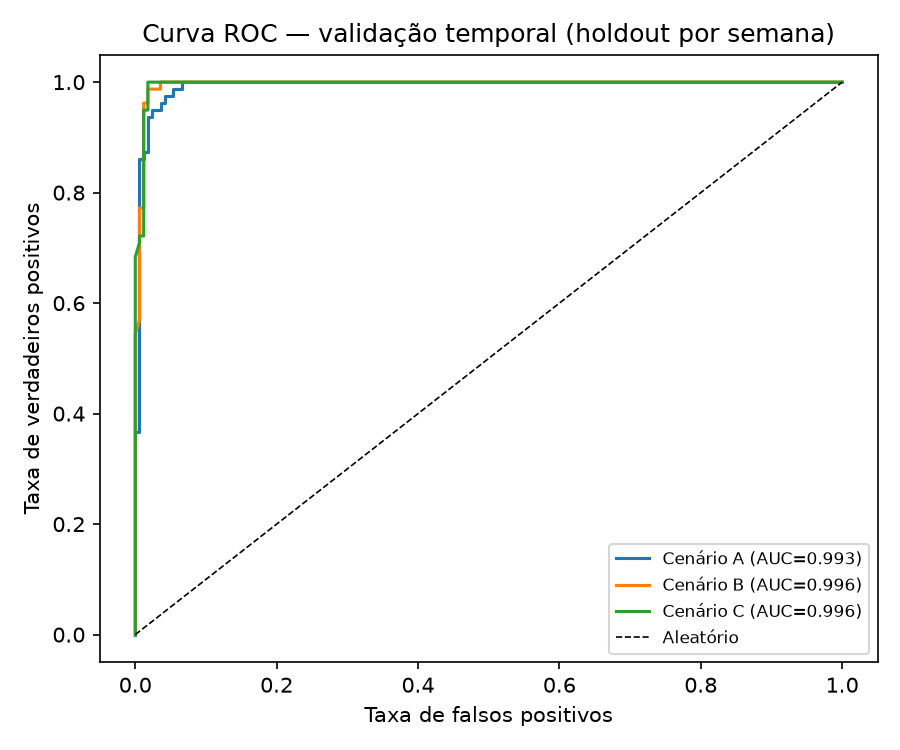
\includegraphics[width=0.7\textwidth]{figuras/fig_roc.png}
\caption{Curvas ROC dos três cenários sob validação temporal.}
\end{figure}

\begin{figure}[h]
\centering
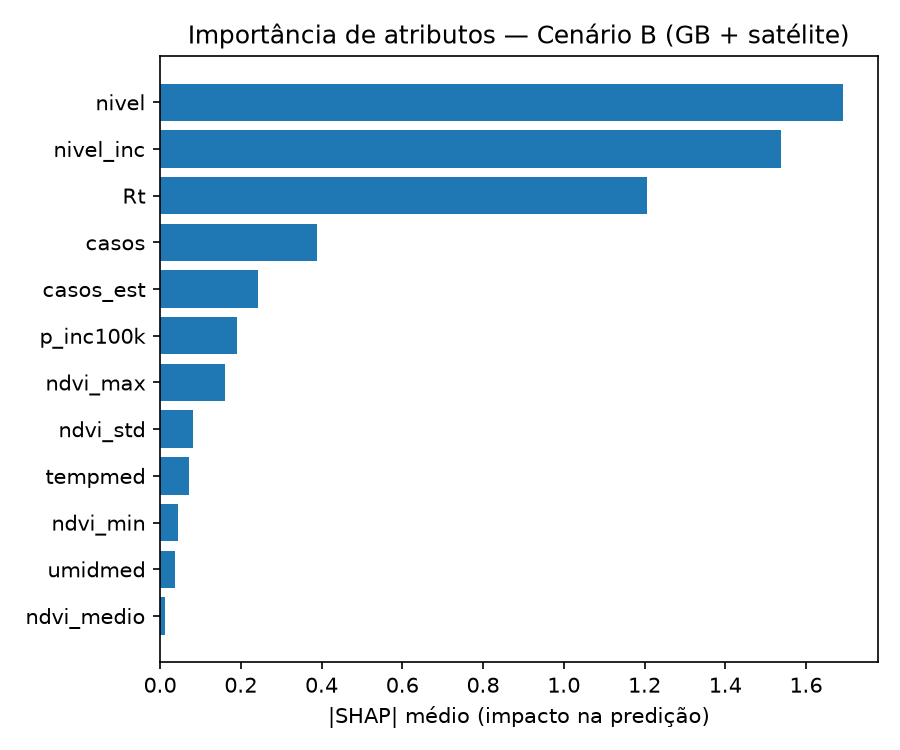
\includegraphics[width=0.7\textwidth]{figuras/fig_shap.png}
\caption{Importância de atributos (SHAP) no cenário B.}
\end{figure}

\begin{table}[h]
\centering
\caption{Importância SHAP (|valor| médio) — cenário B, oito principais.}
\begin{tabular}{lr}
\toprule
Atributo & |SHAP| médio \\
\midrule
    nivel & 1,69243 \\
    nivel\_inc & 1,53750 \\
    Rt & 1,20528 \\
    casos & 0,38952 \\
    casos\_est & 0,24262 \\
    p\_inc100k & 0,18968 \\
    ndvi\_max & 0,16082 \\
    ndvi\_std & 0,08097 \\
\bottomrule
\end{tabular}
\end{table}

\section{Discussão}
A interpretação mecanicista é direta: os atributos de nível de alerta e
persistência (\texttt{nivel}, \texttt{nivel\_inc}, \texttt{Rt}) dominam o SHAP,
e o NDVI aparece abaixo deles. Isso é coerente com o resultado nulo: quando a
informação epidemiológica recente já está disponível, a vegetação acrescenta
pouco. Por que o NDVI não ajudou? Prováveis razões: (i) a resolução temporal do
composto de 16 dias é grosseira frente à dinâmica semanal; (ii) o NDVI médio do
município dilui micro-habitats urbanos do vetor; (iii) a agregação espacial por
fronteira municipal não captura heterogeneidade intraurbana.

\section{Limitações}
\begin{enumerate}
\item Cobertura de 8 capitais; não representa o território nacional.
\item O composto de 16 dias e a defasagem conservadora reduzem a sensibilidade temporal.
\item Subnotificação heterogênea do InfoDengue, maior em regiões periféricas.
\item NDVI médio municipal não resolve a escala do habitat do \emph{Aedes}.
\end{enumerate}

\section{Impacto mais amplo}
Todos os dados são públicos e abertos (InfoDengue, NASA, IBGE); o custo de
computação é nulo. O estudo reforça a soberania de dados públicos brasileiros e
discute o viés de subnotificação. Divulgamos que o manuscrito foi gerado por
sistema de IA com curadoria humana.

\section{Declaração de uso de IA}
Texto e código produzidos por pipeline multiagente com roteamento MoE; o papel
humano foi curadoria, definição da hipótese e validação. Zero dados sintéticos.

\begin{thebibliography}{99}
\bibitem{10.1371/journal.pntd.0005973} Guo, Pi; Liu, Tao; Zhang, Qin; Wang, Li; Xiao, Jianpeng; Zhang, Qingying. Developing a dengue forecast model using machine learning: A case study in China. PLOS Neglected Tropical Diseases, v. 11, p. e0005973, 2017. DOI: 10.1371/journal.pntd.0005973.
\bibitem{10.1073/pnas.1909865116} Johansson, Michael A.; Apfeldorf, Karyn M.; Dobson, Scott; Devita, Jason; Buczak, Anna L.; Baugher, Benjamin. An open challenge to advance probabilistic forecasting for dengue epidemics. Proceedings of the National Academy of Sciences, v. 116, p. 24268-24274, 2019. DOI: 10.1073/pnas.1909865116.
\bibitem{10.1371/journal.pntd.0008056} Zhao, Naizhuo; Charland, Katia; Carabali, Mabel; Nsoesie, Elaine O.; Maheu-Giroux, Mathieu; Rees, Erin. Machine learning and dengue forecasting: Comparing random forests and artificial neural networks for predicting dengue burden at national and sub-national scales in Colombia. PLOS Neglected Tropical Diseases, v. 14, p. e0008056, 2020. DOI: 10.1371/journal.pntd.0008056.
\bibitem{10.1038/srep33707} Johansson, Michael A.; Reich, Nicholas G.; Hota, Aditi; Brownstein, John S.; Santillana, Mauricio. Evaluating the performance of infectious disease forecasts: A comparison of climate-driven and seasonal dengue forecasts for Mexico. Scientific Reports, v. 6, 2016. DOI: 10.1038/srep33707.
\bibitem{10.1016/j.physa.2019.121266} Chakraborty, Tanujit; Chattopadhyay, Swarup; Ghosh, Indrajit. Forecasting dengue epidemics using a hybrid methodology. Physica A: Statistical Mechanics and its Applications, v. 527, p. 121266, 2019. DOI: 10.1016/j.physa.2019.121266.
\bibitem{10.1371/journal.pntd.0005729} Marques-Toledo, Cecilia de Almeida; Degener, Carolin Marlen; Vinhal, Livia; Coelho, Giovanini; Meira, Wagner; Codeço, Claudia Torres. Dengue prediction by the web: Tweets are a useful tool for estimating and forecasting Dengue at country and city level. PLOS Neglected Tropical Diseases, v. 11, p. e0005729, 2017. DOI: 10.1371/journal.pntd.0005729.
\bibitem{10.1371/journal.pntd.0010509} Nguyen, Van-Hau; Tuyet-Hanh, Tran Thi; Mulhall, James; Minh, Hoang Van; Duong, Trung Q.; Chien, Nguyen Van. Deep learning models for forecasting dengue fever based on climate data in Vietnam. PLOS Neglected Tropical Diseases, v. 16, p. e0010509, 2022. DOI: 10.1371/journal.pntd.0010509.
\bibitem{10.3390/ijerph17020453} Xu, Jiucheng; Xu, Keqiang; Li, Zhichao; Meng, Fengxia; Tu, Taotian; Xu, Lei. Forecast of Dengue Cases in 20 Chinese Cities Based on the Deep Learning Method. International Journal of Environmental Research and Public Health, v. 17, p. 453, 2020. DOI: 10.3390/ijerph17020453.
\bibitem{10.1098/rsif.2016.0410} Yamana, Teresa K.; Kandula, Sasikiran; Shaman, Jeffrey. Superensemble forecasts of dengue outbreaks. Journal of The Royal Society Interface, v. 13, 2016. DOI: 10.1098/rsif.2016.0410.
\bibitem{10.1016/j.sste.2020.100372} Mussumeci, Elisa; Codeço Coelho, Flávio. Large-scale multivariate forecasting models for Dengue - LSTM versus random forest regression. Spatial and Spatio-temporal Epidemiology, v. 35, p. 100372, 2020. DOI: 10.1016/j.sste.2020.100372.
\bibitem{10.1038/s41598-020-79193-2} Salim, Nurul Azam Mohd; Wah, Yap Bee; Reeves, Caitlynn; Smith, Madison; Yaacob, Wan Fairos Wan; Mudin, Rose Nani. Prediction of dengue outbreak in Selangor Malaysia using machine learning techniques. Scientific Reports, v. 11, 2021. DOI: 10.1038/s41598-020-79193-2.
\bibitem{10.1186/s12879-019-3874-x} Jain, Raghvendra; Sontisirikit, Sra; Iamsirithaworn, Sopon; Prendinger, Helmut. Prediction of dengue outbreaks based on disease surveillance, meteorological and socio-economic data. BMC Infectious Diseases, v. 19, 2019. DOI: 10.1186/s12879-019-3874-x.
\bibitem{10.1371/journal.pone.0152688} Ramadona, Aditya Lia; Lazuardi, Lutfan; Hii, Yien Ling; Holmner, Åsa; Kusnanto, Hari; Rocklöv, Joacim. Prediction of Dengue Outbreaks Based on Disease Surveillance and Meteorological Data. PLOS ONE, v. 11, p. e0152688, 2016. DOI: 10.1371/journal.pone.0152688.
\bibitem{10.1371/journal.pntd.0010631} Leung, Xing Yu; Islam, Rakibul M.; Adhami, Mohammadmehdi; Ilic, Dragan; McDonald, Lara; Palawaththa, Shanika. A systematic review of dengue outbreak prediction models: Current scenario and future directions. PLOS Neglected Tropical Diseases, v. 17, p. e0010631, 2023. DOI: 10.1371/journal.pntd.0010631.
\bibitem{10.4081/gh.2019.771} Anno, Sumiko; Hara, Takeshi; Kai, Hiroki; Lee, Ming-An; Chang, Yi; Oyoshi, Kei. Spatiotemporal dengue fever hotspots associated with climatic factors in Taiwan including outbreak predictions based on machine-learning. Geospatial Health, v. 14, 2019. DOI: 10.4081/gh.2019.771.
\bibitem{10.1371/journal.pone.0189988} Buczak, Anna L.; Baugher, Benjamin; Moniz, Linda J.; Bagley, Thomas; Babin, Steven M.; Guven, Erhan. Ensemble method for dengue prediction. PLOS ONE, v. 13, p. e0189988, 2018. DOI: 10.1371/journal.pone.0189988.
\bibitem{10.1186/s12879-018-3066-0} Carvajal, Thaddeus M.; Viacrusis, Katherine M.; Hernandez, Lara Fides T.; Ho, Howell T.; Amalin, Divina M.; Watanabe, Kozo. Machine learning methods reveal the temporal pattern of dengue incidence using meteorological factors in metropolitan Manila, Philippines. BMC Infectious Diseases, v. 18, 2018. DOI: 10.1186/s12879-018-3066-0.
\bibitem{10.1016/j.actatropica.2018.05.003} Scavuzzo, Juan M.; Trucco, Francisco; Espinosa, Manuel; Tauro, Carolina B.; Abril, Marcelo; Scavuzzo, Carlos M.. Modeling Dengue vector population using remotely sensed data and machine learning. Acta Tropica, v. 185, p. 167-175, 2018. DOI: 10.1016/j.actatropica.2018.05.003.
\bibitem{10.1016/j.artmed.2021.102157} Hoyos, William; Aguilar, Jose; Toro, Mauricio. Dengue models based on machine learning techniques: A systematic literature review. Artificial Intelligence in Medicine, v. 119, p. 102157, 2021. DOI: 10.1016/j.artmed.2021.102157.
\bibitem{10.1371/journal.pone.0270933} Dey, Samrat Kumar; Rahman, Md. Mahbubur; Howlader, Arpita; Siddiqi, Umme Raihan; Uddin, Khandaker Mohammad Mohi; Borhan, Rownak. Prediction of dengue incidents using hospitalized patients, metrological and socio-economic data in Bangladesh: A machine learning approach. PLOS ONE, v. 17, p. e0270933, 2022. DOI: 10.1371/journal.pone.0270933.
\bibitem{10.1016/j.eswa.2021.116324} Souza, Caio; Maia, Pedro; Stolerman, Lucas M.; Rolla, Vitor; Velho, Luiz. Predicting dengue outbreaks in Brazil with manifold learning on climate data. Expert Systems with Applications, v. 192, p. 116324, 2022. DOI: 10.1016/j.eswa.2021.116324.
\bibitem{10.1038/s41598-024-52796-9} Sebastianelli, Alessandro; Spiller, Dario; Carmo, Raquel; Wheeler, James; Nowakowski, Artur; Jacobson, Ludmilla Viana. A reproducible ensemble machine learning approach to forecast dengue outbreaks. Scientific Reports, v. 14, 2024. DOI: 10.1038/s41598-024-52796-9.
\bibitem{10.1186/s12911-021-01493-y} Yavari Nejad, Felestin; Varathan, Kasturi Dewi. Identification of significant climatic risk factors and machine learning models in dengue outbreak prediction. BMC Medical Informatics and Decision Making, v. 21, 2021. DOI: 10.1186/s12911-021-01493-y.
\bibitem{10.1101/046193} Codeço, Cláudia T; Cruz, Oswaldo G; Riback, Thais I; Degener, Carolin M; Gomes, Marcelo F; Villela, Daniel. InfoDengue: a nowcasting system for the surveillance of dengue fever transmission. 2016. DOI: 10.1101/046193.
\bibitem{10.1016/j.respe.2018.05.408} Codeco, C.; Coelho, F.; Cruz, O.; Oliveira, S.; Castro, T.; Bastos, L.. Infodengue: A nowcasting system for the surveillance of arboviruses in Brazil. Revue d'Épidémiologie et de Santé Publique, v. 66, p. S386, 2018. DOI: 10.1016/j.respe.2018.05.408.
\bibitem{10.1201/b13040-9} Shimabukuro, Yosio Edemir; dos Santos, João Roberto; Formaggio, Antonio Roberto; Duarte, Valdete; Theodor Rudorff, Bernardo Friedrich. The Brazilian Amazon Monitoring Program: PRODES and DETER Projects. Global Forest Monitoring from Earth Observation, p. 153-169, 2016. DOI: 10.1201/b13040-9.
\bibitem{10.1016/j.rse.2017.06.031} Gorelick, Noel; Hancher, Matt; Dixon, Mike; Ilyushchenko, Simon; Thau, David; Moore, Rebecca. Google Earth Engine: Planetary-scale geospatial analysis for everyone. Remote Sensing of Environment, v. 202, p. 18-27, 2017. DOI: 10.1016/j.rse.2017.06.031.
\bibitem{10.1023/A:1010933404324} Breiman, Leo. Random Forests. Machine Learning, v. 45, p. 5-32, 2001. DOI: 10.1023/A:1010933404324.
\bibitem{10.1145/2382577.2382579} Kaufman, Shachar; Rosset, Saharon; Perlich, Claudia; Stitelman, Ori. Leakage in data mining. ACM Transactions on Knowledge Discovery from Data, v. 6, p. 1-21, 2012. DOI: 10.1145/2382577.2382579.
\bibitem{10.1111/j.1365-2656.2008.01390.x} Elith, J.; Leathwick, J. R.; Hastie, T.. A working guide to boosted regression trees. Journal of Animal Ecology, v. 77, p. 802-813, 2008. DOI: 10.1111/j.1365-2656.2008.01390.x.
\bibitem{10.1017/s0950268821001801} Queiroz, Eny Regina da Silva; Medronho, Roberto de Andrade. Spatial analysis of the incidence of Dengue, Zika and Chikungunya and socioeconomic determinants in the city of Rio de Janeiro, Brazil. Epidemiology and Infection, v. 149, 2021. DOI: 10.1017/s0950268821001801.
\bibitem{10.1016/j.tmaid.2025.102934} Bermudi, Patricia Marques Moralejo; Palasio, Raquel Gardini Sanches; Pirani, Monica; Santana, Lidia Maria Reis; Barbosa, Gerson Laurindo; Blangiardo, Marta. Dengue incidence, mortality, and case-fatality in Brazil: spatial patterns, socioeconomic contrasts, and serotype impact. Travel Medicine and Infectious Disease, v. 68, p. 102934, 2025. DOI: 10.1016/j.tmaid.2025.102934.
\bibitem{10.3390/rs14195052} Li, Zhichao; Dong, Jinwei. Big Geospatial Data and Data-Driven Methods for Urban Dengue Risk Forecasting: A Review. Remote Sensing, v. 14, p. 5052, 2022. DOI: 10.3390/rs14195052.
\bibitem{10.1080/01431160902865756} Fuller, Douglas O.; Troyo, Adriana; Calderón-Arguedas, Olger; Beier, John C.. Dengue vector (<i>Aedes aegypti</i>) larval habitats in an urban environment of Costa Rica analysed with ASTER and QuickBird imagery. International Journal of Remote Sensing, v. 31, p. 3-11, 2010. DOI: 10.1080/01431160902865756.
\bibitem{10.1016/j.srs.2026.100490} Singh, Shubham K.; Fan, Peilei; Chen, Jiquan. Ecoregion-specific dengue risk prediction in Peru using remote sensing, machine learning, and spatiotemporal modeling. Science of Remote Sensing, v. 14, p. 100490, 2026. DOI: 10.1016/j.srs.2026.100490.
\bibitem{10.1016/j.ecoinf.2020.101149} Brum-Bastos, Vanessa; Long, Jed; Church, Katharyn; Robson, Greg; de Paula, Rogério; Demšar, Urška. Multi-source data fusion of optical satellite imagery to characterize habitat selection from wildlife tracking data. Ecological Informatics, v. 60, p. 101149, 2020. DOI: 10.1016/j.ecoinf.2020.101149.
\bibitem{10.21203/rs.3.rs-3161529/v1} Lima, Hélder; Tupinambás, Unaí; Guimarães, Frederico. Estimating epidemiological parameters and underreporting of Covid-19 cases in Brazil using a multi-wave mathematical model. 2023. DOI: 10.21203/rs.3.rs-3161529/v1.
\bibitem{10.3390/tropicalmed7100322} Cabrera, Maritza; Leake, Jason; Naranjo-Torres, José; Valero, Nereida; Cabrera, Julio C.; Rodríguez-Morales, Alfonso J.. Dengue Prediction in Latin America Using Machine Learning and the One Health Perspective: A Literature Review. Tropical Medicine and Infectious Disease, v. 7, p. 322, 2022. DOI: 10.3390/tropicalmed7100322.
\bibitem{10.18280/ria.370521} Thirugnanam, Archana; Hussain, Faritha Banu Jahir. Exploring Machine Learning Algorithms for the Prediction of Dengue: A Comprehensive Review. Revue d'Intelligence Artificielle, v. 37, p. 1281-1290, 2023. DOI: 10.18280/ria.370521.
\bibitem{10.31449/inf.v43i3.1548} Iqbal, Naiyar; Islam, Mohammad. Machine learning for dengue outbreak prediction: A performance evaluation of different prominent classifiers. Informatica, v. 43, 2019. DOI: 10.31449/inf.v43i3.1548.
\end{thebibliography}

\end{document}
